\chapter{SymmSAT}\label{chap:symmSAT}


This chapter presents our first contribution published in TACAS 2018 conference~\ref{algorithm:cdcl_cosy}. 

\section{General idea}
%\subsubsection{Drawbacks of the static-based approaches.} 
In the general case,
the size of the \textit{sbp} can be exponential in the number of variables of
the problem so that they cannot be totally computed. Even in more favorable
situations, the size of the generated \textit{sbp} is often too large to be
effectively handled by a SAT solver~\cite{Luks2004}. On the other hand, if
only a subset of the symmetries is considered then the resulting search pruning
will not be that interesting and its effectiveness depends heavily on the
heuristically chosen symmetries \cite{biere2009handbook}. Besides, these approaches
are preprocessors, so their combination with other techniques, such as
\emph{symmetry propagation}~\cite{Devriendt12}, can be very hard. Also, tuning
their parameters during the solving turns out to be very difficult. For all
these reasons, some classes of SAT problems cannot be solved yet despite
the presence of symmetries.
To handle these issues, we propose a new
approach that reuses the principles of the static approaches, but operates
dynamically: the symmetries are broken during the search process without any
pre-generation of the \textit{sbp}. It is a best effort approach that tries to eliminate,
\textit{dynamically}, the \textit{non lex-leading} assignments with a minimal
computation effort. To do so, we first introduce the notions of
\textit{reducer}, \textit{inactive} and \textit{active} permutation with
respect to an assignment $\alpha$ and \emph{effective symmetric breaking predicates} (\emph{esbp}).


\begin{definition}[Reducer, inactive and active permutation]
	 A permutation $g$	is a \emph{reducer} of an assignment $\alpha$ if $g.\alpha < \alpha$ 
	 (hence $\alpha$ cannot be the lex-leader of its orbit. $g$ reduces it and all its extensions). $g$ is
	\emph{inactive} on $\alpha$ when $\alpha < g.\alpha$ (so, $g$ cannot reduce $\alpha$ and all
	the extensions). A symmetry is said to be \emph{active} with respect to $\alpha$
	when it is neither inactive nor a reducer of $\alpha$. 
\end{definition}

Proposition~\ref{prop:status} restates this definition in terms of variables
and is the basis of an efficient algorithm to keep track of the status of a
permutation during the solving. Let us, first, recall that the \emph{support}
 of a permutation $g$, $\support_g$, the set $\{ v \in \Vars \mid g.v \neq v\}$.

\begin{proposition}
	\label{prop:status}
	Let $\alpha \in \Assignments(\Vars)$ be an assignment, $g \in \Group$ a permutation and $ \support_g \subseteq  \Vars$ the support of $g$. We say that $g$ is:
	\begin{enumerate}
		\item  \emph{a reducer of} $\alpha$  if there exists a variable $v \in \Vars_g$
		such that:
		\begin{itemize}
			\item $\forall\ v' \in \Vars_g$, s. t. $v' \prec v$, either $\{v', g^{-1}(v')\}\subseteq\alpha $ or $\{\neg v', \neg g^{-1}(v')\} \subseteq \alpha $,
			\item $\{v, \neg g^{-1}(v)\} \subseteq \alpha$;
		\end{itemize}
		\item  \emph{inactive} on $\alpha$  if there exists a variable $v \in \Vars_g$
		such that:
		\begin{itemize}
			\item $\forall\ v' \in \Vars_g$, s. t. $v' \prec v$, either $\{v', g^{-1}(v')\}\subseteq\alpha $ or $\{\neg v', \neg g^{-1}(v')\} \subseteq \alpha $,
			\item $\{\neg v, g^{-1}(v)\} \subseteq \alpha$;
		\end{itemize}
		\item  \emph{active} on $\alpha$, otherwise.
	\end{enumerate}
\end{proposition}

When $g$ is a \textit{reducer} of $\alpha$ we can define a predicate that contradicts $\alpha$ yet preserves the satisfiability of the formula. Such a predicate will be used to discard $\alpha$, and all its extensions, from a further visit and hence pruning the search tree.

\begin{definition}[Effective Symmetry Breaking Predicate]
	\label{def:esbp}
	Let $\alpha \in \Assignments(\Vars)$, and $g \in \Group{\Vars}$.
	We say that the formula $\psi$ is an effective symmetry breaking predicate (\textit{esbp} for short) for $\alpha$ under $g$ if:
	$$\alpha \not\models \psi \text{ and for all }\beta \in \Assignments(\Vars), \beta \not\models \psi \Rightarrow g.\beta < \beta$$
\end{definition}

The next definition gives a way to obtain such an effective symmetry-breaking predicate from an assignment and a reducer.

\begin{definition}[A construction of an \emph{esbp}]
	\label{def:eta}
	Let $\varphi$ be a formula.
	Let $g$ be a symmetry of $\varphi$ that reduces an assignment $\alpha$.
	Let $v$ be the variable whose existence is given by item 1. in Proposition~\ref{prop:status}.
	Let $U = \{ v', \neg v' \mid v' \in \Vars_g \text{ and } v'~\preceq~v\}$.
	We define $\eta(\alpha, g)$ as $(U \cup g^{-1}.U) \setminus \alpha$.
\end{definition}

\textbf{Example}. Let us consider $\Vars = \{x_1, x_2, x_3, x_4, x_5\}$, $g =
(x_1\,x_3)(x_2\,x_4)$, and a partial assignment $\alpha = \{x_1, x_2,
x_3, \neg x_4\}$. Then, $g.\alpha = \{x_1, \neg x_2, x_3, x_4\}$ and $v = x_2$.
So, $U = \{x_1, \neg x_1, x_2, \neg x_2\}$ and $g^{-1}.U = \{x_3, \neg x_3,
x_4, \neg x_4\}$ and we can deduce than $\eta(\alpha, g) = (U \cup g^{-1}.U)
\setminus \alpha = \{\neg x_1, \neg x_2, \neg x_3, x_4\}$.

\begin{proposition}
	\label{prop:eta}
	$\eta(\alpha, g)$ is an effective symmetry-breaking predicate.
\end{proposition}
\begin{proof}
	It is immediate that $\alpha \not\models \eta(\alpha, g)$.
	
	Let $\beta \in \Assignments(\Vars)$ such that $\beta \wedge \eta(\alpha, g)$ is \unsat. We denote a $\alpha'$
	and $\beta'$ as the restrictions of $\alpha$ and $\beta$ to the variables in $\{ v' \in
	\Vars_g \mid v'~\preceq~v \}$. Since $\beta \wedge \eta(\alpha, g)$ is \unsat, $\alpha' = \beta'$.
	But $g.\alpha' < \alpha'$, and $g.\beta' < \beta'$. By monotonicity of $<$, we thus also have
	$g.\beta < \beta$. \end{proof}

\medskip\noindent It is important to observe that the notion of \textit{ebsp}
is a refinement of the classical concept of \textit{sbp} defined in \cite{aloul06}. In particular, like \textit{sbp}, \textit{esbp} preserve satisfiability.

\begin{theorem}[Satisfiability preservation]
	Let $\varphi$ be a formula and $\psi$ an \textit{esp} for some assignment $\alpha$ under $g \in S(\varphi)$. Then,
	$$\varphi~and ~\varphi \wedge \psi \text{ are equi-satisfiable}.$$
\end{theorem}

\begin{proof}
	
	If $\varphi \wedge \psi$ is SAT then $\varphi$ is trivially SAT. If
	$\varphi$ is SAT, then there is some assignment $\beta$ that satisfies $\varphi$.
	Without loss of generality, $\beta$ can be chosen to be the lex-leader of its
	orbit under $S(\varphi)$. Thus, $g$ does not reduce $\beta$, which implies that
	$\beta \models \psi$.
	
\end{proof}




\subsection{Algorithm}


This section describes how to augment the state-of-the-art CDCL algorithm with
the aforementioned concepts to develop an efficient symmetry-guided SAT
solving algorithm. 
The approach is implemented using a couple of components: (1) a
\textit{Conflict Driven Clauses Learning (CDCL) search engine}; (2) \textit{a symmetry controller}. Roughly speaking, the first component performs the
classical search activity on the SAT problem, while the second observes the
engine and maintains the status of the symmetries. When the controller detects
a situation where the engine is starting to explore a redundant
part\footnote{Isomorphic to a part that has been/will be explored.}, it orders
the engine to operate a backjump. The detection is performed thanks to
\emph{symmetry status tracking} and the backjump order is given by a simple
injection of an \emph{esbp} computed on the fly.
Principle of CDCL is described in section \ref{sec:cdcl}, \cref{algorithm:cdcl_cosy} explains how to extend it with a \emph{symmetry controller} component which guides the behavior of CDCL algorithm depending on the status of symmetries.

\begin{algorithm}[!htbp]
	\SetKwProg{Fn}{function}{}{}
	\SetKwData{C}{SymController}
	\SetKwFunction{CDCL}{CDCLSym}
	\SetKwFunction{unitPropagation}{unitPropagation}
	\SetKwFunction{analyzeConflict}{analyzeConflict}
	\SetKwFunction{addLearntClause}{addLearntClause}
	\SetKwFunction{assignNewLiteral}{assignDecisionLiteral}
	\SetKwFunction{backjumpPolicy}{backjumpAndRestartPolicies}
	\SetKwFunction{isNotMinimal}{isNotLexLeader}
	\SetKwFunction{SBP}{generateEsbp}
	\SetKwFunction{notifyAssigned}{updateAssign}
	\SetKwFunction{notifyCancelled}{updateCancel}
	\SetKwFunction{symmetryController}{symmetryController}

	\DontPrintSemicolon
	
	\Fn{\CDCL{$\varphi$: CNF formula, {\color{red}\C: symmetry controller}}
		\textbf{returns} $\true$ if $\varphi$ is \sat and $\false$ otherwise}
	{
		$dl \gets 0$ \tcp*{Current decision level}
		$\alpha \gets \emptyset$\;
		\While {not all variables are assigned} {
			$isConflict \gets$ \unitPropagation{}\;
			{
				\color{red} 
				\C.\notifyAssigned{$\alpha$}\;\label{algo:cdcl_sym:notify}
				$isReduced \gets$ \C.\isNotMinimal{$\alpha$}\;\label{algo:cdcl_sym:not_minimal}
			}
			
			\If{$isConflict \, {\color{red}||\, isReduced}$} {
				\If{dl == 0}
				{
					\Return \false
					\tcp*{$\varphi$ is $\unsat$}
				}
				\If{\color{red}$isConflict$}
				{
					$\omega \gets$ \analyzeConflict{}\;
				}
				\Else {
					{
						\color{red}$\omega \gets$ \C.\SBP{$\alpha$}\;\label{algo:cdcl_sym:gen_esbp}
					}
				}
			$\varphi \gets \varphi \cup \{\omega$\} \;
				$dl \gets$ \backjumpPolicy{}\;
				{\color{red}\C.\notifyCancelled{$\alpha$}\;} \label{algo:cdcl_sym:cancel}
			}
			\Else{
				$\alpha \gets \alpha\, \cup $ \assignNewLiteral{}\; 
			$dl \gets dl+1$\;
			}
		}
		\Return \true
		\tcp*{$\varphi$ is $\sat$}
		
	}
	\caption{the CDCLSym SAT Solving Algorithm.}
	\label{algorithm:cdcl_cosy}
\end{algorithm}


 
 The symmetry controller is initially given a set of symmetries $G$ \footnote{The generators of the group of symmetries.}. It observes the behavior of the SAT engine and updates its internal data according to the current assignment, to keep track of the status of the symmetries. This observation is \emph{incremental}: whenever a literal is assigned or cancelled, the symmetry controller updates the status of all the symmetries. This corresponds to \cref{algo:cdcl_sym:notify,algo:cdcl_sym:cancel} of Algorithm~\ref{algo:cdcl}. When the controller detects that the
 current assignment can not be a \emph{lex-leader} (\cref{algo:cdcl_sym:not_minimal}), it generates the
 corresponding \emph{esbp} (\cref{algo:cdcl_sym:gen_esbp}).
 
 \medskip\noindent In the remainder of this section, functions
 composing the symmetry controller are detailed.
 
 \subsubsection{Symmetries Status Tracking.} The \texttt{updateAssign},
 \texttt{updateCancel} and \texttt{isNot\-LexLeader} functions (\Cref{algo:keep_status}) track the status of symmetries based on
 Proposition~\ref{prop:status} ; there, resides th  core of our algorithm.
 
 All these functions rely on the $\track$ structure: a map of variables indexed
 by permutations. Initially, $\track[g] = \min_{\prec}(\support_g)$ for all $g \in G$ according to the ordering relation and all
 permutations are marked \textit{active}.
 
 For each permutation, $g$, the symmetry controller keeps track of the smallest
 variable $\track[g]$ in the support of $g$ such that $\track[g]$ and
 $g^{-1}(\track[g])$ do not have the same value in the current assignment. If
 one of the two variables is not assigned, they are considered not to have the
 same value.
 
 When new literals are assigned, only active symmetries need to have their
 $\track[g]$ updated (line $2$). This update is done thanks to a while
 loop (lines $4-5$).
 
 When literals are cancelled, we need to update the status of symmetries for
 which some variable $v$ before $\track[g]$, or $g^{-1}(v)$, becomes unassigned
 (lines $9-10$). Symmetries that were inactive may be reactivated (line $11$).
 
 The current assignment is not a \textit{lex-leader} if some symmetry $g$ is a
 reducer. This is detected by comparing the value of $\track[g]$ with the value
 of $g^{-1}(\track[g])$ (line $16$). The function \texttt{isNotLexLeader} also
 marks symmetries as \emph{inactive} when appropriate (lines $18-19$).
 
 \subsubsection{Generation of the \emph{esbp}.} When the current assignment
 cannot be a \textit{lex-leader}, some symmetry $g$ is a reducer. The function
 \texttt{generateEsbp} computes the $\eta(\alpha, g)$ defined in~\Cref{def:eta},
 which is an effective symmetry-breaking predicate by~\Cref{prop:eta}. This will
 prevent the SAT engine to explore further the current partial assignment.
 
 \begin{algorithm}[!htbp]
	\SetKwProg{Fn}{function}{}{}
 	\SetKwFunction{notifyAssigned}{updateAssign}
 	
 	\Fn{\notifyAssigned{$\alpha$: assignment}
 	}{
 		\ForEach{active $g \in  G$}{
 			$v \gets \track[g]$\;
 			\While{ $\{v, g^{-1}(v)\}\subseteq\alpha $ \textbf{or} $\{\neg v, \neg g^{-1}(v)\} \subseteq\alpha$ }{
 				$v \gets$ next variable in $\Vars_g$\;
 			}
 			$\track[g] \gets v$
 		}
 	}
 	
 	\Fn{\notifyCancelled{$\alpha$: assignment}}{
 		\ForEach{$g \in G$}{
 			$u \gets \min \{ v \in \Vars_g \mid \{v, \neg v\} \cap \alpha = \emptyset \text{ or } \{g^{-1}(v), \neg g^{-1}(v)\} \cap \alpha = \emptyset \}$\;
 			\If{$u \preceq \track[g]$}{
 				mark $g$ as active\;
 				$\track[g] \gets u$\;
 			}
 			
 		}
 	}
 	
 	
 	\Fn{\isNotMinimal{$\alpha$: assignment}}{
 		\ForEach{active $g \in G$}{
 			$v \gets \track[g]$\;
 			\If{$\{v, \neg g^{-1}(v)\}\subseteq\alpha$} {
 				\Return \true 	\tcp*{$g$ is a reducer}
 			}
 			\If{$\{\neg v, g^{-1}(v)\}\subseteq\alpha$}{
 				mark $g$ as inactive
 				\tcp*{$g$ can't reduce $\alpha$ or its extentions}
 			}
 			
 		}
 		\Return \false
 	}
 	
 	
 	\Fn{\SBP{$\alpha$: assignment} \textbf{returns} $\omega$: generated $esbp$}
 	{
 		$\omega \gets \{\}$\;
 		$g \gets$ the reducer of $\alpha$ detected in \isNotMinimal\;
 		$v \gets min(\Vars_g)$\;
 		$u \gets \track[g] $\;
 		\While{$u \neq v$}{
 			\leIf{$v \in \alpha$} {$\omega \gets \omega \cup \{\neg v\}$}{$\omega \gets \omega \cup \{v\}$}
 			\leIf{$g^{-1}(v) \in \alpha$} {$\omega \gets \omega \cup \{\neg g^{-1}(v)\}$}{$\omega \gets \omega \cup \{g^{-1}(v)\}$}
 			$v \gets$ next variable in $\Vars_g$
 		}
 		$\omega \gets \omega \cup \{\neg v, g^{-1}(v)\}$\;
 		\Return $\omega$
 	}
 	\caption{the functions keeping track of the status of the symmetries and generating the \emph{esbp}.}
 	\label{algo:keep_status}
 	
 \end{algorithm}
 
 
 
 \subsection{Illustrative example}
  Let us illustrate the previous concepts and algorithms on a simple example. Let the ordering relation $x_1 \prec x_2 \prec x_3 \prec x_4
 \prec x_5 \prec x_6\ \mid \false < \true$, and the two last previous generators
 $G = \{
 	g_2 = (x_1 \enskip x_2)(x_4 \enskip x_5),g_3 = (x_1 \enskip x_4)(x_2 \enskip x_5)(x_3 \enskip x_6)\}$
 (written in cycle notation with opposite cycles omitted). Their
 respective supports sorted according to ordering relation are, $\support_{g_{2}} = \{x_1, x_2, x_4, x_5\}$ and
 $\support_{g_3} = \{x_1, x_2, x_3, x_4, x_5, x_6\}$.
 
 On the assignment $\alpha = \emptyset$, both permutations are active and
 $\track[g_1] = \track[g_2] = x_1$. When the solver updates the assignment to $\alpha = \{ x_4\}$, both permutations remain active and $\track[g_2] = \track[g_3] = x_1$. On the assignment $\alpha = \{  x_4,  x_1\}$, the symmetry controller updates $\track[g_3]$ to $x_2$, while $\track[g_2]$ remains unchanged. On the assignment $\alpha = \{  x_4,  x_1, \neg x_2 \}$, $g_2.\alpha = \{  x_5,  x_2, \neg x_1
 \}$, which is smaller than $\alpha$ (because $ x_1 \in \alpha$ and $ \neg x_1 \in g.\alpha$):
 $g_2$ is a reducer of $\alpha$. The symmetry controller then generates the
 corresponding \textit{esbp} $\omega = \{ \neg x_1, x_2 \}$.
 
 
\section{Implementation and Evaluation}\label{sec:eval}

In this section, we first highlight some details on our implementation of the
symmetry controller. Then, we experimentally assess the performance of our
algorithm against three other state-of-the-art tools.

\subsection{\libdsb{}: an efficient implementation of the symmetry controller}

We have implemented our method in a C++ library called \libdsb{} (1630 LoC). It
implements a symmetry controller as described in the previous section, and can
be interfaced with virtually any CDCL SAT solver. \libdsb{} is released under
GPL~v3 licence and is available at \url{https://github.com/lip6/cosy}.

\subsubsection{Heuristics and Options.} Let us recall that finding the optimal
ordering of variables (with respect to the exploitation of symmetries) is
NP-hard~\cite{luks.04.amai}, so the choice for this ordering is heuristic.
\libdsb{} offers several possibilities to define this ordering:

\begin{itemize}
	
	\item a naive ordering, where variables are ordered by the lexicographic
	order of their names;
	
	\item an ordering based on occurrences, where variables are sorted
	according to the number of times they occur in the input formula. The
	lexicographic order of variables names is used for those having the same number of
	occurrences;
	
	\item an ordering based on symmetries, where variables belonging to the
	same orbit (under the given set of symmetries) are grouped together. Orbit are
	ordered by their numbers of occurrences.
	
\end{itemize}

The ordering of assignments we use in this paper orders positive literals
before negative ones (thus, $\true < \false$), but using the converse
ordering does not change the overall method. However, it can impact the
performance of the solver on some instances, so that it is an option of the
library.

All the symmetries we used for the presentation of our approach are
permutations of variables. Our method straightforwardly extends to permutations of literals, also known as \emph{value permutations} \cite{biere2009handbook}.


\subsubsection{Integration in \minisat{}.} We show how to integrate \libdsb{}
to an existing solver, through example of \minisat{}~\cite{een2003extensible}.

First, we need an adapter that allows the communication between the solver and
\libdsb{} (30 LoC). Then, we adapt Algorithm \ref{algo:cdcl} to the different
methods and functions of \minisat{}. In particular, the function
\texttt{updateAssign} is moved into the \texttt{uncheckEnqueue} function of
\minisat{} (2 LoC). The \texttt{updateCancel} function is moved to the
\texttt{cancelUntil} function of \minisat{} that performs the backjumps (2
LoC). The \texttt{isNotLexLeader} and \texttt{generateEsbp} functions are
integrated in the \texttt{propagate} function of \minisat{} (30 LoC). This is
to keep track of the assignments as soon as they occur, then the
\textit{esbp} is produced as soon as an assignment is identified as not being
\emph{lex-leader}. Initialization issues are located in the main function of
\minisat (15 LoC).

The integration of \libdsb{} increases \minisat{} code by~3\%.
 

\subsection{Evaluation}

% \textcolor{red}{revoir le commentaire lorsqu'on aura tous les tableaux...}
%
% \textcolor{red}{rajouter un paragraphe sur une expérience pour lever le doute
% sur le fait que nos perfs soient liees a un effet de bord d'implementation.
% Essayer de lancer notre outil avec l'ordre d'un autre outil. On ferait une
% analyse en quelques lignes en indiquant la variablite observee. Experience =
% ordre true/false + l'ordre de breakID.}

This section presents the evaluation of our approach. All experiments have been
performed with our modified \minisat{} called \cdclsym{}. The symmetries of the
SAT problem instances have been computed by two different state-of-the-art
tools \saucy{}~\cite{katebi2010symmetry} and
\bliss{}~\cite{JunttilaKaski:ALENEX2007}. For a given group of symmetries, the
first tool generates less permutations to represent the group than the second
one, but it is slower than the other one.

We selected from the last six editions of the SAT contests
\cite{jarvisalo2012international}, the CNF instances for which \bliss{} finds
at least 2\% of the variables are involved in some symmetries that could be
computed in at most $1000s$ of CPU time. We obtained a total of $1350$
symmetric instances (discarding repetitions) out of $3700$ instances in total.

All experiments have been conducted using the following conditions: each solver
has been run once on each instance, with a time-out of 5000 seconds (including
the execution time of the symmetries generation except for \minisat) and limited
to 8GB of memory. Experiments were executed on a computer with an Intel Xeon
X7460 2.66 GHz featuring 24 cores and 128GB of memory, running a Linux 4.4.13,
along with g++ compiler version 6.3.

We compare \cdclsym{} using the occurrence order, value symmetries, and without
\emph{lex-leader} forcing, against:

\begin{itemize}
	
	\item \minisat{}, as the reference solver without symmetry handling
	\cite{een2003extensible};
	
	\item \shatter{}, a symmetry breaking preprocessor described in \cite{aloul06},
	coupled with the \minisat{} SAT engine;
	
	\item \breakid{}, another symmetry breaking preprocessor, described in
	\cite{Devriendt16}, also coupled with the \minisat{} SAT engine.
	
\end{itemize}

Each \sat solution was successfully checked against the initial CNF. For \unsat
situations, there is no way to provide an \unsat certificate in presence of
symmetries. Nevertheless, we checked our results were also computed by the
other measured tools. Unfortunately, out of the 1350 benchmarked formulas, we
have no proof or evidence for the 15 \unsat formulas computed by \cdclsym{}
only.

Results are presented Tables in~\ref{table:benchUNSAT}, \ref{table:benchSAT},
and \ref{tab:par2}. We report the number of instances solved within the time
and memory limits for each solver and category. We separate the UNSAT instances
(\Cref{table:benchUNSAT}) from the SAT ones (\Cref{table:benchSAT}). Besides
the reference with no symmetry (column \minisat{}), we have compared the
performance of the three tools when using symmetries computed by \saucy{} (see
Table~\ref{table:unsat:saucy} and Table~\ref{table:sat:saucy}), and \bliss{}
(see Table~\ref{table:unsat:bliss} and Table~\ref{table:sat:bliss}). Rows
correspond to groups of instances: from each edition of the SAT contest, and
when possible, we separated applicative instances (app$\langle x \rangle$ where
$\langle x \rangle$ indicates the year) from hard combinatorial ones
(hard$\langle x \rangle$). This separation was not possible for the editions
2015 and 2017 (all2015 and all2017). The total number of instances for each
bench is indicated between parentheses. For each row, the cells corresponding
to the tools solving the most instances (within time and memory limits) are
typeset in bold and greyed out. Table~\ref{tab:par2} shows the cumulative and
average PAR-2 times of the evaluated tools.

\begin{table}[t]
	\resizebox{1 \textwidth}{!}{
		\subfloat[With \saucy]{%
			\begin{tabular}{l|ccccc}
				Benchmark  &\texttt{MiniSAT} & \texttt{Shatter} & \texttt{BreakID} & \texttt{MiniSym}\\
				\midrule
				app2016 (134) & 18 & 19 & \cellcolor{gray!30}\textbf{20} & 17\\
				app2014 (161) & 23 & 23 & 22 & \cellcolor{gray!30}\textbf{24}\\
				app2013 (145) & 6 & 8 & 8 & \cellcolor{gray!30}\textbf{10}\\
				app2012 (367) & 115 & 115 & \cellcolor{gray!30}\textbf{120} & \cellcolor{gray!30}\textbf{120}\\
				\hline
				hard2016 (128) & 8 & 17 & \cellcolor{gray!30}\textbf{50} & 42\\
				hard2014 (107) & 9 & 24 & \cellcolor{gray!30}\textbf{30} & 29\\
				hard2013 (121) & 12 & 24 & \cellcolor{gray!30}\textbf{48} & 29\\
				hard2012 (289) & 86 & 84 & 88 & \cellcolor{gray!30}\textbf{93}\\
				\hline
				all2017 (124) & 8 & 14 & \cellcolor{gray!30}\textbf{15} & 14\\
				all2015 (65) & 9 & 8 & 8 & \cellcolor{gray!30}\textbf{10}\\
				\hline
				TOTAL (no dup)  & 261 & 302 & \cellcolor{gray!30}\textbf{371} & 345\\
				\label{table:unsat:saucy}
			\end{tabular}
		}
		\hspace{1em}
		\subfloat[With \bliss]{%
			\begin{tabular}{l|ccccc}
				Benchmark  &\texttt{MiniSAT} & \texttt{Shatter} & \texttt{BreakID} & \texttt{MiniSym}\\
				\midrule
				app2016 (134) & 18 & \cellcolor{gray!30}\textbf{21} & 18 & 19\\
				app2014 (161) & 23 & 21 & 20 & \cellcolor{gray!30}\textbf{24}\\
				app2013 (145) & 6 & 7 & 10 & \cellcolor{gray!30}\textbf{11}\\
				app2012 (367) & 115 & 106 & 114 & \cellcolor{gray!30}\textbf{123}\\
				\hline
				hard2016 (128) & 8 & 11 & \cellcolor{gray!30}\textbf{79} & 77\\
				hard2014 (107) & 9 & 45 & 40 & \cellcolor{gray!30}\textbf{53}\\
				hard2013 (121) & 12 & 51 & \cellcolor{gray!30}\textbf{56} & 54\\
				hard2012 (289) & 86 & 69 & 90 & \cellcolor{gray!30}\textbf{93}\\
				\hline
				all2017 (124) & 8 & 14 & \cellcolor{gray!30}\textbf{15} & \cellcolor{gray!30}\textbf{15}\\
				all2015 (65) & \cellcolor{gray!30}\textbf{9} & 7 & 8 & 8\\
				\hline
				TOTAL (no dup) & 261 & 324 & 415 & \cellcolor{gray!30}\textbf{439}\\
				\label{table:unsat:bliss}
			\end{tabular}
		}
	}
	\vspace*{0.1cm}
	\caption{comparison of different approaches on the \unsat instances of the benchmarks of the six last editions of the SAT competition.}
	\label{table:benchUNSAT}
\end{table}

\begin{table}
	\resizebox{1 \textwidth}{!}{
		\subfloat[With \saucy]{%
			\begin{tabular}{l|ccccc}
				Benchmark  &\texttt{MiniSAT} & \texttt{Shatter} & \texttt{BreakID} & \texttt{MiniSym}\\
				\midrule
				app2016 (134) & 20 & \cellcolor{gray!30}\textbf{22} & 21 & 20\\
				app2014 (161) & \cellcolor{gray!30}\textbf{24} & \cellcolor{gray!30}\textbf{24} & \cellcolor{gray!30}\textbf{24} & 22\\
				app2013 (145) & 34 & 35 & 35 & \cellcolor{gray!30}\textbf{43}\\
				app2012 (367) & 121 & 112 & 119 & \cellcolor{gray!30}\textbf{126}\\
				\hline
				hard2016 (128) & \cellcolor{gray!30}\textbf{0} & \cellcolor{gray!30}\textbf{0} & \cellcolor{gray!30}\textbf{0} & \cellcolor{gray!30}\textbf{0}\\
				hard2014 (107) & 14 & \cellcolor{gray!30}\textbf{17} & \cellcolor{gray!30}\textbf{17} & 14\\
				hard2013 (121) & 23 & 23 & \cellcolor{gray!30}\textbf{24} & 22\\
				hard2012 (289) & 135 & 141 & \cellcolor{gray!30}\textbf{143} & 138\\
				\hline
				all2017 (124) & 23 & 20 & 26 & \cellcolor{gray!30}\textbf{27}\\
				all2015 (65) & \cellcolor{gray!30}\textbf{7} & 5 & \cellcolor{gray!30}\textbf{7} & 6\\
				\hline
				TOTAL (no dup)  & 325 & 323 & \cellcolor{gray!30}\textbf{337} & 335\\
				\label{table:sat:saucy}
				
			\end{tabular}
		}
		\hspace{1em}
		\subfloat[With \bliss]{%
			\begin{tabular}{l|ccccc}
				Benchmark  &\texttt{MiniSAT} & \texttt{Shatter} & \texttt{BreakID} & \texttt{MiniSym}\\
				\hline
				app2016 (134) & 20 & 20 & \cellcolor{gray!30}\textbf{22} & 20\\
				app2014 (161) & \cellcolor{gray!30}\textbf{24} & \cellcolor{gray!30}\textbf{24} & 23 & 22\\
				app2013 (145) & \cellcolor{gray!30}\textbf{34} & 32 & 30 & 33\\
				app2012 (367) & \cellcolor{gray!30}\textbf{121} & 112 & 120 & 118\\
				\hline
				
				hard2016 (128) & \cellcolor{gray!30}\textbf{0} & \cellcolor{gray!30}\textbf{0} & \cellcolor{gray!30}\textbf{0} & \cellcolor{gray!30}\textbf{0}\\
				hard2014 (107) & 14 & 14 & 17 & \cellcolor{gray!30}\textbf{18}\\
				hard2013 (121) & 23 & 24 & \cellcolor{gray!30}\textbf{26} & 25\\
				hard2012 (289) & 135 & 134 & 141 & \cellcolor{gray!30}\textbf{142}\\
				\hline
				all2017 (124) & 23 & 25 & 26 & \cellcolor{gray!30}\textbf{29}\\
				all2015 (65) & \cellcolor{gray!30}\textbf{7} & 5 & 6 & 6\\
				\hline
				TOTAL (no dup) & 325 & 316 & 334 & \cellcolor{gray!30}\textbf{336}\\
				\label{table:sat:bliss}
			\end{tabular}
		}
	}
	\vspace*{0.1cm}
	\caption{comparison of different approaches on the \sat instances of the benchmarks of the six last editions of the SAT competition.}
	\label{table:benchSAT}
\end{table}

\begin{table}[h!]
	\centering\footnotesize
	\subfloat[With \saucy]{%
		\begin{tabular}{l|c|c}
			Solver & PAR-2 sum & PAR-2 avg \\
			\hline
			\texttt{MiniSAT} & 8\,074\,348       & 5\,981        \\
			\texttt{Shatter} & 7\,770\,434        & 5\,756        \\
			\cellcolor{gray!30}\texttt{BreakID} & \cellcolor{gray!30}6\,909\,999      & \cellcolor{gray!30}5\,119 \\
			\texttt{MiniSym} & 7\,229\,700           & \ 5\,355       
			\label{par2-saucy}
		\end{tabular}
	}
	\hspace{1em}
	\subfloat[With \bliss]{%
		\begin{tabular}{l|c|c}
			Solver & PAR-2 sum & PAR-2 avg \\
			\hline
			\texttt{MiniSAT} & 8\,074\,348        & 5\,981        \\
			\texttt{Shatter} & 7\,517\,556        & 5\,569        \\
			\texttt{BreakID} & 6\,444\,954        & 4\,774        \\ 
			\cellcolor{gray!30}\texttt{MiniSym} & \cellcolor{gray!30}6\,245\,448        & \cellcolor{gray!30}\ 4\,626       
			\label{par2-bliss}
		\end{tabular}
	}
	\vspace*{0.1cm}
	\caption{comparison of PAR-2 times (in seconds) of the benchmarks on the six last editions of the SAT competition.}
	\label{tab:par2}
\end{table}

We observe that \cdclsym{} with \saucy{} solves the most instances in only half
of the \unsat categories. However, with \bliss{}, \cdclsym{} solves the most
instances in all but four of the \unsat categories ; it then also solves the
highest number of instances among its competitors. This shows the interest
of our approach for \unsat instances. Since symmetries are used to reduce the
search space, we were expecting that it will bring the most performance gain
for \unsat instances.

The situation for \sat instances is more mitigated (Table~\ref{table:benchSAT}),
especially when using \saucy{}. Again, this is not very surprising: our method
may cut the exploration of a satisfying assignment because it is not a
\textit{lex-leader}. This delays the discovery of a satisfying assignment. The
other tools suffer less from such a delay, because they rely on symmetry
breaking predicates generated in a pre-processing step. Also, when seeing the
global results of \minisat{}, we can globally state that the use of symmetries
in the case of satisfiable instances only offers a marginal improvement.

\begin{figure}[!htbp]
	\centering
	\subfloat[with \saucy]{{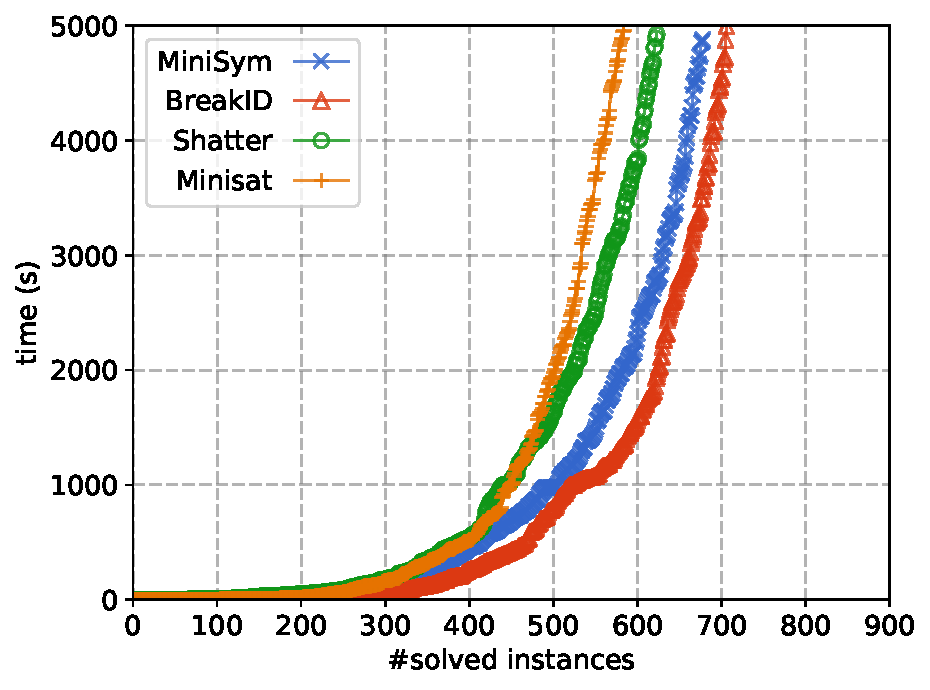
\includegraphics[scale=0.36]{img/saucy-result}}}%
	\qquad
	\subfloat[with \bliss]{{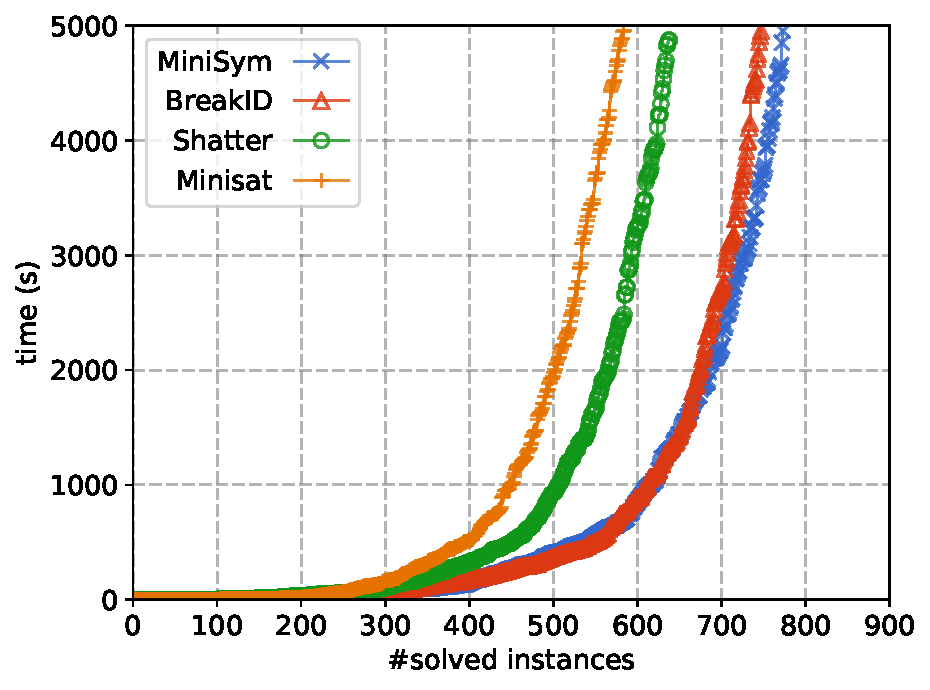
\includegraphics[scale=0.36]{img/bliss-result}}}%
	\caption{cactus plot  total number of instances}%
	\label{fig:cactus}%
\end{figure}

We observe that performances our tool are better with \bliss{} than with
\saucy{} (see fig~\ref{fig:cactus}). We explain it as follows: \saucy{} is
known to compute fewer generators for the group of symmetries than \bliss{}.
Since, the larger the symmetries set is, the earlier the detection of an
\emph{evidence} that an assignment is not a \textit{lex-leader} will be, we
generate less symmetry-breaking predicates (only the effective ones). This is
shown in Table~\ref{tab:sbp}; \cdclsym{} generates an order of magnitude fewer
predicates than \breakid{}.


\begin{table}[!htbp]
	\resizebox{1 \textwidth}{!}{
		\subfloat[With \saucy]{%
			\begin{tabular}{l|c|c}
				Number of SBPs & \texttt{BreakID}  & \texttt{MiniSym}\\
				\hline
				\unsat (316)	& 12\,088\,433  & \cellcolor{gray!30}1\,579\,623 \\
				\sat  (312)    & 13\,839\,689  & \  \cellcolor{gray!30}359\,352     
				\label{sbp-saucy}
			\end{tabular}
		}
		\hspace{1em}
		\subfloat[With \bliss]{%
			\begin{tabular}{l|c|c}
				Number of SBPs & \texttt{BreakID}  & \texttt{MiniSym}\\
				\hline
				\unsat (399)	&  2\,576\,349 &  \cellcolor{gray!30}913\,339\\
				\sat  (320) & 12\,179\,513  & \  \cellcolor{gray!30}457\,452 
				\label{sbp-bliss}
			\end{tabular}
		}
	}
	\vspace*{0.1cm}
	\caption{Comparison of the number of generated SBPs each time \breakid{} and 
		\cdclsym{} both compute a verdict (number of verdicts between parentheses).}
	\label{tab:sbp}
\end{table}

We also conducted experiments on highly symmetrical instances (all variables
are involved in symmetries), whose results are presented
in~\Cref{table:bench2}. The performance of \breakid{} on this benchmark is
explained by a specific optimization for the \emph{total symmetry groups} that
are found in these examples, that is neither implemented in \shatter{} nor in
\cdclsym{}. However, the difference between \breakid{} and \cdclsym{} is rather
thin when using $\bliss{}$. Our tool still outperforms \shatter{} on this
benchmark.

\begin{table}[!htbp]
	\resizebox{1 \textwidth}{!}{
		\subfloat[With \saucy]{%
			\begin{tabular}{l|cccc}
				Benchmark  & \minisat{} & \shatter{} & \breakid{} & \cdclsym{} \\
				\hline
				battleship(6) & \cellcolor{gray!30}\textbf{5} &\cellcolor{gray!30}\textbf{5} & \cellcolor{gray!30}\textbf{5} & \cellcolor{gray!30}\textbf{5}\\
				chnl(6) &  4 & \cellcolor{gray!30}\textbf{6} & \cellcolor{gray!30}\textbf{6} & \cellcolor{gray!30}\textbf{6}\\
				clqcolor(10)  &  3 & 4 & 5 & \cellcolor{gray!30}\textbf{6} \\
				fpga(10) &   6 & \cellcolor{gray!30}\textbf{10} & \cellcolor{gray!30}\textbf{10} & \cellcolor{gray!30}\textbf{10}\\
				hole(24) &   10 & 12 & \cellcolor{gray!30}\textbf{23} & 11\\
				hole shuffle(12)  &  1  & 2 & \cellcolor{gray!30}\textbf{12} & 3\\
				urq(6) &   1  & 2 & \cellcolor{gray!30}\textbf{6} & 2\\
				xorchain(2)  &  1 & 1 & \cellcolor{gray!30}\textbf{2} & \cellcolor{gray!30}\textbf{2} \\
				\hline
				TOTAL & 31 & 42 & \cellcolor{gray!30}\textbf{69} & 45\\
			\end{tabular}
		}
		\hspace{1em}
		\subfloat[With \bliss]{%
			\begin{tabular}{l|cccc}
				Benchmark  & \minisat{} & \shatter{} & \breakid{} & \cdclsym{} \\
				\hline
				battleship(6) & 5 & 5 & 5 & \cellcolor{gray!30}\textbf{6} \\
				chnl(6) &  4 &  \cellcolor{gray!30}\textbf{6} & \cellcolor{gray!30}\textbf{6} & \cellcolor{gray!30}\textbf{6} \\
				clqcolor(10)  &  3 & 5 & 8 & \cellcolor{gray!30}\textbf{10} \\
				fpga(10) &   6 & \cellcolor{gray!30}\textbf{10} & \cellcolor{gray!30}\textbf{10} & \cellcolor{gray!30}\textbf{10} \\
				hole(24) &   10 &\cellcolor{gray!30}\textbf{24} & \cellcolor{gray!30}\textbf{24} & 23 \\
				hole shuffle(12)  &  1  &  3 & \cellcolor{gray!30}\textbf{7} & 4\\
				urq(6) &   1  & 2 & \cellcolor{gray!30}\textbf{6} & 5\\
				xorchain(2)  &  1 & 1 & \cellcolor{gray!30}\textbf{2} & \cellcolor{gray!30}\textbf{2}\\
				\hline
				TOTAL & 31 & 56 & \cellcolor{gray!30}\textbf{68} & 66 \\
			\end{tabular}
		}
	}
	\vspace*{0.1cm}
	\caption{comparison of the tools on 76 highly symmetric $\unsat$ problems.}
	\label{table:bench2}
\end{table}


\section{Conclusion}

SymmSAT uses same principles as static symmetry breaking but operates dynamically by 
injecting effective symmetry breaking during the search.
This overcomes, the main problem of the static approaches , that they
generate many \textit{sbp} that are not effective in the solving (size of the
generated formulas, overburden of the unit propagation procedure, etc.).
The idea we bring is to break symmetries \emph{on the fly}: when the current
partial assignment can not be a prefix of a \textit{lex-leader} (of an orbit),
an \textit{esbp} that prunes this forbidden assignment and all its extensions is generated. 

This approach is implemented in the C++ library called \libdsb{}. It is an
off-the-shelf component that can be interfaced with virtually any CDCL SAT
solver. \libdsb{} is released under GPL licence and is available at
\url{https://github.com/lip6/cosy}.
 
The extensive evaluation of our approach on the symmetric formulas of the last
six SAT contests shows that it outperforms the state-of-the-art techniques, in
particular on unsatisfiable instances, which are the hardest class of the
problem.




